\documentclass[tikz,border=10pt]{standalone}
\usepackage{tikz}
\usetikzlibrary{positioning}

\begin{document}

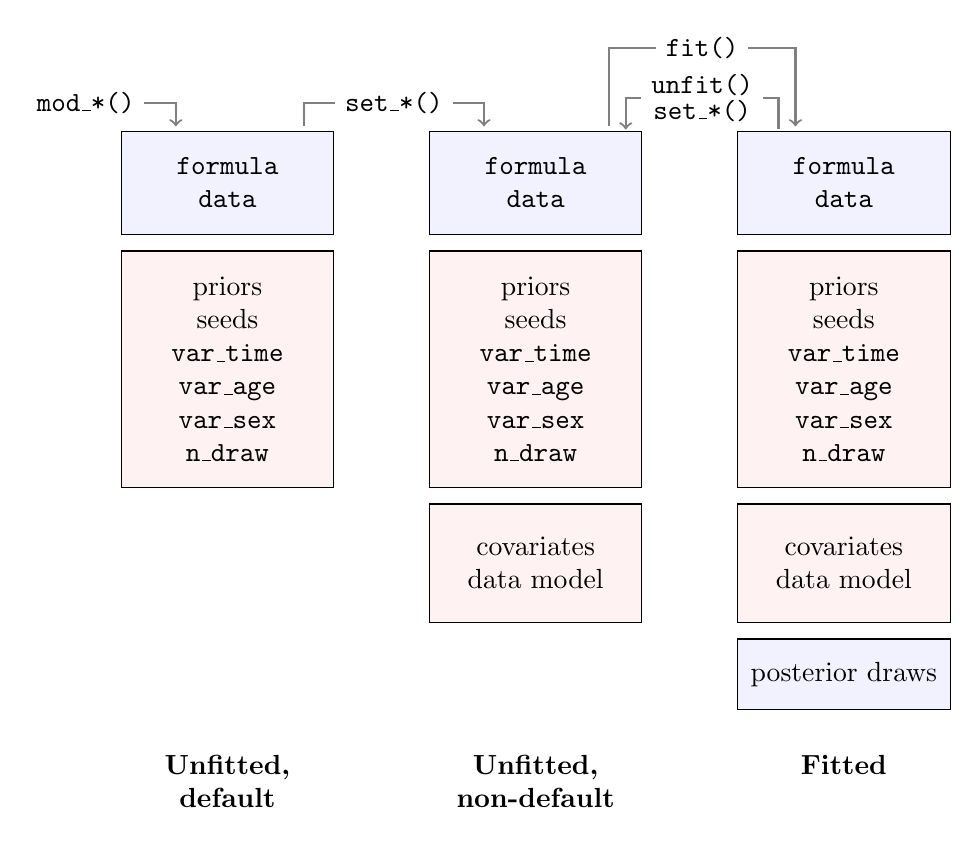
\begin{tikzpicture}

  \usetikzlibrary{shapes.geometric}
  \usetikzlibrary{shapes.symbols}
  
  % Unfitted, defaults

  \node[draw, rectangle, minimum width=2.7cm, minimum height=1.3cm, align=center, fill = blue!5!] (box1a) {\texttt{formula} \\ \texttt{data}};
    \node[below=7.8cm, font=\bfseries, align = center] at (box1a.north) {Unfitted, \\ default};
    
    \node[draw, rectangle, minimum width=2.7cm, minimum height=3cm, align=center, below=2mm of box1a, fill = red!5!] (box2a) {priors \\ seeds \\ \texttt{var\_time} \\ \texttt{var\_age} \\ \texttt{var\_sex} \\ \texttt{n\_draw}};

    %  Unfitted, non-default
    
    \node[draw, rectangle, minimum width=2.7cm, minimum height=1.3cm, align=center, right=1.2cm of box1a, fill = blue!5!] (box1b) {\texttt{formula} \\ \texttt{data}};
    \node[below=7.8cm, font=\bfseries, align = center] at (box1b.north) {Unfitted, \\ non-default};

    \node[draw, rectangle, minimum width=2.7cm, minimum height=3cm, align=center, below=2mm of box1b, fill = red!5!] (box2b) {priors \\ seeds \\ \texttt{var\_time} \\ \texttt{var\_age} \\ \texttt{var\_sex} \\ \texttt{n\_draw}};

    \node[draw, rectangle, minimum width=2.7cm, minimum height=1.5cm, align=center, below=2mm of box2b, fill = red!5!] (box3b) {covariates \\ data model};

    % Fitted

    \node[draw, rectangle, minimum width=2.7cm, minimum height=1.3cm, align=center, right=1.2cm of box1b, fill = blue!5!] (box1c) {\texttt{formula} \\ \texttt{data}};
    \node[below=7.8cm, font=\bfseries, align = center] at (box1c.north) {Fitted};

    \node[draw, rectangle, minimum width=2.7cm, minimum height=3cm, align=center, below=2mm of box1c, fill = red!5!] (box2c) {priors \\ seeds \\ \texttt{var\_time} \\ \texttt{var\_age} \\ \texttt{var\_sex} \\ \texttt{n\_draw}};

    \node[draw, rectangle, minimum width=2.7cm, minimum height=1.5cm, align=center, below=2mm of box2c, fill = red!5!] (box3c) {covariates \\ data model};

    \node[draw, rectangle, minimum width=2.7cm, minimum height=0.9cm, align=center, below=2mm of box3c, fill = blue!5!] (box4c) {posterior draws};


% Function mod
    \node[above=1mm of box1a, xshift = -1.8cm, align = center, font=\tt](f-unfitted)  {mod\_*()};
    \draw[->,thick, gray] (f-unfitted.east) -| +(4mm, -3mm);

 % Function set
    \node[above=1mm of box1b, xshift = -1.8cm, align = center, font=\tt](f-unfitted-nondefault)  {set\_*()};
    \draw[thick,gray] (f-unfitted-nondefault.west) -| +(-4mm, -3mm);
    \draw[->,thick,gray] (f-unfitted-nondefault.east) -| +(4mm, -3mm);

% Function fit
    \node[above=8mm of box1c, xshift = -1.8cm, align = center, font=\tt](f-fit)  {fit()};
    \draw[thick,gray] (f-fit.west) -| +(-6mm, -10mm);
    \draw[->,thick,gray] (f-fit.east) -| +(6mm, -10mm);

% Function unfit,set
  \node[above=0mm of box1c, xshift = -1.8cm, align = center, font=\tt](f-unfit)  {unfit() \\[-1mm] set\_*()};
  \draw[->,thick,gray] (f-unfit.west) -| +(-2mm, -4mm);
  \draw[thick,gray] (f-unfit.east) -| +(2mm, -4mm);


\end{tikzpicture}

\end{document}


